\documentclass[letter, 11pt]{article}

% Need to do some more reading: http://plain-text.co/pull-it-together.html
% Convert from LaTeX to Markdown:
% pandoc --standalone --wrap=none --base-header-level=2 -f latex -t gfm+smart+citations --filter=pandoc-citeproc --bibliography=Geopyter.bib --csl=apalike.csl -M Title="GeoPyTeR: Mashable (Geography) Teaching Resources for Python" -B header.md Geopyter.tex -o README.md

\newcommand{\gp}{\textsc{g}eo\textsc{p}y\textsc{t}e\textsc{r}~\/}
\newcommand{\eg}{e.g.~\/}
\newcommand{\ie}{i.e.~\/}
\newcommand{\comment}[1]{\todo[inline, color=green!40]{#1}}

%% Language and font encodings
\usepackage[english]{babel}
\usepackage[utf8x]{inputenc}
\usepackage[T1]{fontenc}
\usepackage[hyphens]{url}
\usepackage{fancyvrb} % facny verbatim
\usepackage{textcomp}
\usepackage{upquote}  % Turns quotes in verbatim to straight
\usepackage{varioref} % for vpageref[above]
\usepackage{fullpage}
\usepackage{graphicx} 
\usepackage[font=small,labelfont=bf]{caption}
%% Sets page size and margins
%\usepackage[letter,top=3cm,bottom=2cm,left=3cm,right=3cm,marginparwidth=1.75cm]{geometry}

%% For citations
%\usepackage{natbib}
\usepackage[%
% numberedbib,
  natbibapa
]{apacite} 

%% Useful packages
\usepackage{amsmath}
\usepackage[colorinlistoftodos]{todonotes}
\usepackage[colorlinks=false, allcolors=black]{hyperref}
\def\tightlist{}

\title{Geographical Python Teaching Resources: GeoPyTeR}
\author{Jonathan Reades \and Sergio Rey}

\begin{document}
\maketitle

\begin{abstract}
  Abstract goes here.
\end{abstract}


\section{Introduction}\label{introduction}

Although \citet{Donoho2017} traces the origins of data science back to
\citeauthor{Tukey1962}'s \textit{The future of data analysis}
(\citeyear{Tukey1962}), its emergence has led to a flourishing of tools and
programmes as universities seek to engage with this nascent---and
lucrative---interdisciplinary field. One of the most profound practical impacts
of this development has been on the ways in which developers share and execute
code: although systems for combining code, commentary, and results have been
around for some time (\eg R-Markdown) these were intended primarily for
replicating research outputs, not for the online teaching of a new technique or
writing of an interactive introduction to a software library. The `open' ethos
and rapid growth of data science, and the need for a lightweight interactive
code-sharing platform mean that teachers in many disciplines are playing
catch-up on both the methods taught and the formats used.

As a discipline, geography has been acutely aware of these developments: changes
in the volume and extent of geographical data available (\eg
\citealp{Graham2013,gonzalez2013big,reades2016}), and in the number and range of
methods employed to identify patterns in those data (\eg
\citealp{Fan2016,Naik2017,Santibanez2015,Stevens2015,ArribasBel2017}), are
allowing us to tackle questions thought unanswerable just a few years ago. At
the same time, however, there is growing evidence of a `hollowing out' of
traditional domain-specific skills: most of what a trained geographer used to do
with specialist software can now be done using free online resources (\eg
Google's Fusion Tables, MapBox, Carto, ArcOnline), but there remains unmet
demand for graduates who can \textit{code} in order to take advantage of the
latest (geo)algorithms and techniques \citep{Singleton2014,Singleton2016}.

\section{Statement of Need}

Regardless of whether this is a revolution \citep{Wyly2014,Torrens2010} or an
evolution \citep{Barnes2013,Barnes2014,ArribasBel2018}, there is no question
that teaching students and researchers how to code and how to \textit{think}
computationally presents new challenges
\citep{Etherington2016,Muller2014,rey_09jgs}. Specifically, because of the way
that these changes have unfurled, the majority of resources used in the
classroom are being developed from scratch at each institution, and often by
newly-appointed lecturers and assistant professors coming from the relatively
small number of elite research facilities active in this domain (see discussion
in \citealp{esrc2013}). Not only has this led to the duplication of effort at
multiple sites, but it has also had an enormous impact on the productivity---as
commonly measured by institutions---of early career researchers, many of whom
are in their first teaching post.

The overarching purpose of this software is therefore to address two seemingly
contradictory issues: the recognition that no two instructors teach in precisely
the same way, and the fact that few instructors have the luxury of both time and
tenure to develop compelling new course material in splendid isolation. This
where the Geographical Python Teaching Resource
(\textsc{g}eo\textsc{p}y\textsc{t}e\textsc{r}) comes into play: although
developed with geographers in mind, it provides a generic means by which
instructors in any discipline can selectively incorporate and re-mix programming
and conceptual content from existing Jupyter notebooks while providing their own
`gloss' for this content. Our approach therefore seeks to develop a richer, open
community of developers and teachers who work \textit{together} on new teaching
materials, and to support instructors in quickly adapting existing materials to
new delivery formats.

\section{Origins and Inspirations}\label{origins-and-inspirations}

Like many open source projects, \gp grew out of a need to scratch an itch: in
our roles as teachers of (geo)computational concepts and methods we grappled on
an annual basis with the demands of developing and updating instructional
material with complex interdependencies. And, while the fundamental computing
and analytic concepts may remain fairly stable, the field is highly-dynamic in
terms of both the content and the rate of evolution of new features in
contributed code upon which we rely for functionality. Currently, every time a
widely-used library package is updated a protracted sequence of revisions
ensues: some teachers, pressed for time, may resist making use of---or even
alerting students to---the new features; others may leap in enthusiastically,
only to discover that they hadn't fully thought through the challenges of
conflicting dependencies and evolving feature sets.

We initially explored with others---faculty with whom we regularly
collaborate---the potential to `divide and conquer': we would each focus on
different topics and then combine these contributions to create a full course.
Though received with some enthusiasm, this plan did not survive contact with
reality: first, when actually faced with the uncertain promise of receiving a
full course in return for our efforts, many of us felt more secure developing
our own material; second, we had underestimated the value that we each attach to
the ability to personalise material to our own style of teaching. Since the
shared materials were being developed individually according to the individual's
own `style', any rationalisation or personalisation would have to be done by the
instructor at a later date and without support from the rest of the project.

Going back to the drawing board, we looked again at our own experiences of
successful programming and instructional efforts. In particular, we took note of
two powerful streams of thought in software and education: the importance
attached by the Free and Open Source Software (\textsc{foss}) movement to both
peer-recognition \citep{raymond_cathedral_1999} and distributed version control;
and the rise of Virtual Learning Environments (\textsc{vle}s) and of Massive
Open Online Courses (\textsc{mooc}s) with their use of rich, online learning
experiences (\eg \citealp{Trafford2011,Cabiria2012}). Reflecting on our initial
failure, we decided against trying to supply a single set of polished course
materials and instead looked for a way to provide teachers with building blocks
from which they could assemble an \textit{individualised} course suited to their
institutional and pedagogical needs.

We drew inspiration from the \textsc{foss} iPython project
\citep{perez_2007_ipython} and its transformative impact on the sharing of
integrated code, text, and multimedia resources. And we also looked to the
Python Spatial Analysis Library (\textsc{p}y\textsc{sal}) project
\cite{rey_19sea}in which contributors take ownership of application areas
through managed collaboration instead of a contributory `free-for-all'. The
subsequent emergence of the Jupyter project \cite{kluyver16} from iPython has
led to the rapid growth of a rich ecosystem of tools that support the kinds of
interaction needed to make this an effective teaching resource:
multiuser-notebooks (jupyterhub), automation of grading (nbgrader), interactive
widgets for visualisation (ipywidgets), and packages to facilitate manipulation
of the notebook itself (nbformat and notebook).

With these criteria and resources in mind, we began looking for ways to lower
the `entry costs' for faculty to both take from, and share into, the corpus of
instructional material, as well as for a way to address the
customisation/localisation challenge. \gp was our solution: a single, open hub
of teaching concepts and practical programming tasks that can be flexibly
assembled into classes, or entire courses! In the \gp approach we recognise that
teachers need to be able to develop their own classroom `story' at their own
pace (and in conformance with their institution's teaching pattern), while
supporting them with a library of up-to-date materials from which they can pick
and choose. So in much the same way that a computer application is compiled from
the contributions of many developers, \gp allows individual classes and entire
courses to be `compiled' from the contributions of many skilled teachers and
developers.

\section{System Architecture}\label{system-architecture}

At least in our experience, the pace of technological and methodological change
is such that the gap between what instructors know and what students know is
substantial, and in many cases might even be growing. The differences within
individual student cohorts may be greater still, however, and while students
need to be able to begin their learning `journey' at some arbitrary point in the
progression from `learning to code' towards `computational social scientist'
\citep{Lazer2009}, instructors require the ability to assemble a course that
meets students where they \emph{are} rather than where the instructor or
institution might \emph{wish} them to be.

The guiding insight behind \gp is that instruction in computation proceeds from
fundamental units of learning typically built around \textit{computing} concepts
(variables, lists/arrays, dictionaries/hashes, functions/subroutines, etc.) to
fundamental units of learning built around \textit{analytic} concepts (cluster
analysis, point patterns, spatial autocorrelation, etc.). These units must then
be assembled in a way that speaks to the student cohort and its background; we
mean this in two ways: first, that the examples used must speak to budding
geographers, political scientists, historians, etc.; and second, that it should
be possible to develop courses for different cohorts without having to start
over from scratch. In other words, how can we enable teachers to reuse many of
the building blocks employed in an advanced course for Masters students in an
introductory undergraduate course?

\subsection{Components}\label{components}

From these constraints it was clear that our system needed to support a
`bottom-up' approach to instructional design. So although the development of a
course or class could---and probably should---start with a clear set of learning
aims and outcomes, at a certain point the instructor will be searching for a
examples with which to teach a particular concept: What \emph{is} a list or
dictionary? What is \textit{k}-means clustering? We settled on the term `Atoms'
to refer to these basic instructional units and, much like entries in the atomic
table, we felt that they could be grouped together into sets of related
concepts: the fundamentals of programming, point pattern analysis, machine
learning, etc.

Each atom would employ \emph{domain-specific} illustrative examples and code so
as to anchor learning in relevant problems and applications. An atom on arrays
written for geographers could start by showing how these simple data structures
can be used to hold data about cities (\eg name, country, population); but a
subsequent unit could build on this with an an illustration of how nested data
structures allow us to add city location using nested coordinate pairs (\eg
latitude and longitude within an array-of-arrays). This is why managed
collaboration around sets of related concepts is so important: quite aside from
the fact that no \textsc{foss} project succeeds without some level of executive
control, it's critical that \textit{someone} is responsible for ensuring a
degree of consistency in how the units fit together within a set of
closely-related topics.

The purpose of the bottom-up approach is that these units can then be flexibly
assembled into Sessions: from the \textit{same ingredients} (\ie atoms) the
instructor could create two quite different modules---one for delivery in
person, one for delivery online---by organising the elements in different ways.
Quite simply, we don't want to have to rewrite material for each format:
lecture/practical, `flipped' classroom, or \textsc{mooc}. Furthermore, sessions
designed for experts (\eg those pursuing continuing online education) might be
able to `move' students through many more atoms of instruction in a single
session than a similarly laid out (in terms of time) session designed for
first-time programmers in an undergraduate programme. So sessions need to be
able to \emph{incorporate} atoms in a way that minimises the level of effort
involved in finding the `best' way to, for example, explain the concept of
recursion while maximising the ability of the instructor to relate this concept
to the students' practical experience (\eg by providing a `context' that is
anchored in a locally relevant `story' or data).

Naturally, Sessions can then be grouped into Learning Modules (modules) that
offer a coherent instructional programme over a period of weeks or months.
Modules represent the highest level of abstraction in the proposed system, but
they are also obviously the starting point from which instructors can organise
their (remixed) atomic and sessional material into something incorporating a set
of learning outcomes and a package of assessment appropriate to their students.
However, our design reflects the expectation that contributions to \gp at each
\emph{level} of instruction might be made by \emph{different} people: a domain
expert in Spatial Bayes might be the right person to develop an Atom on the
concept and its application, but not the right person to develop a module
tackling advanced spatial analytic concepts where this is just one approach
amongst many. Similarly, given the global diversity of delivery formats, a
10-week term in Britain enables students to cover a very different `volume' of
content from a 15-week American semester. \gp recognises and seeks to respond to
that diversity at all levels.

\subsection{Tools}\label{tools}

So we are trying to design a system in which sessions and modules are
\emph{composed} out of atomic units of instruction that can be, optionally,
surrounded by the instructor's own `narrative' or supported by more locally
relevant (geo)data. We therefore want to produce a set of teaching materials
that are highly portable, easily re-used or edited, and that enable the
instructor to select only the elements from which they wish to compose their
materials. As intimated above, \gp operationalises this through the Jupyter
project and its ability to provide in-browser access to the Python
interpreter\footnote{Other languages are also possible using different kernels;
there is no reason that \gp couldn't be used to create instructional materials
in these languages as well.}, and it also takes advantage of the dominance of
Git and GitHub for version control as a means for tracking authorship across
many versions and changes.

In theory, thanks to the combination of Jupyter and GitHub is not even necessary
for the novice user to have Python installed on their own computer: since all
interaction with Python is via the browser, the environment could be hosted on a
server halfway round the world. In practice, however, there are few such
services and most users simply download and install a free version of Python
(\eg Anaconda) that will run on their system. In our field many people are
already using this approach: notebooks can be found covering everything from
introductory concepts \citep{millington_reades_2017_code} to advanced spatial
analysis methods \citep{darribas_gds15}, and combined for both complete courses
or workshops \citep{rey_2016_narsc}.

Jupyter notebooks are written as a mix of executable code cells and
non-executable text formatted with the widely-used `markdown' syntax. Notebook
structure is provided through headers in markdown cells: a `\#' pre-pended to a
line of text is generally taken to be the title of the notebook; `\#\#' at the
start of a line provides a second level of structure (\ie level 2 headers);
`\#\#\#' indicates level 3 headers; etc. For our purposes, what's relevant is
that these headers yield a natural hierarchy that corresponds closely to the
h1\ldots{}h6 model used by the HTML markup language that lies at the heart of
the World Wide Web. This hierarchy allows us to `abstract out' the problem of
inferring the \emph{meaning} of different sections of the notebook since the
instructor does it for us.

Notebooks are actually stored in a format called JavaScript Object Notation
(\textsc{json}) that is not particularly easy for most humans to read, but as it
is nonetheless highly-structured we can interact with it programmatically. The
extensible nature of the \textsc{json} format also allows us to read and write
both data and metadata not only to each notebook, but also to each and every
sub-element of a notebook. Since metadata that is not understood by Jupyter is
simply ignored, we can add our own fields to provide useful information related
to instruction: the amount of time that the notebook's examples and content
might take to cover in class; who should be given credit for contributing; any
dependencies or requirements for installed libraries\ldots

In short, within the notebook we have two types of structure that can be used
not only to provide information that may assist course instructors in developing
content, but also to uniquely specify a section, subsection, or sub-subsection
of content (code or text) at a fine-grained level. Taken together, this provides
the foundation for a mechanism to select content in one notebook and import it
into another. This therefore creates an opportunity to remix/mash up content
while still being able to add an institutional or course-specific gloss wherever
necessary. Each notebook might start with the instructor's contact information
or by providing instructions for setting up the computing environment, but then
make use of material developed by others for actual instruction. This process
may seem quite abstract---and probably quite convoluted as well---but an
illustration (Figure \ref{fig:Illustration} \vpageref[above]{fig:Illustration})
may help to clarify why this process is so useful.

\begin{figure}[hbtp]
  \centering
  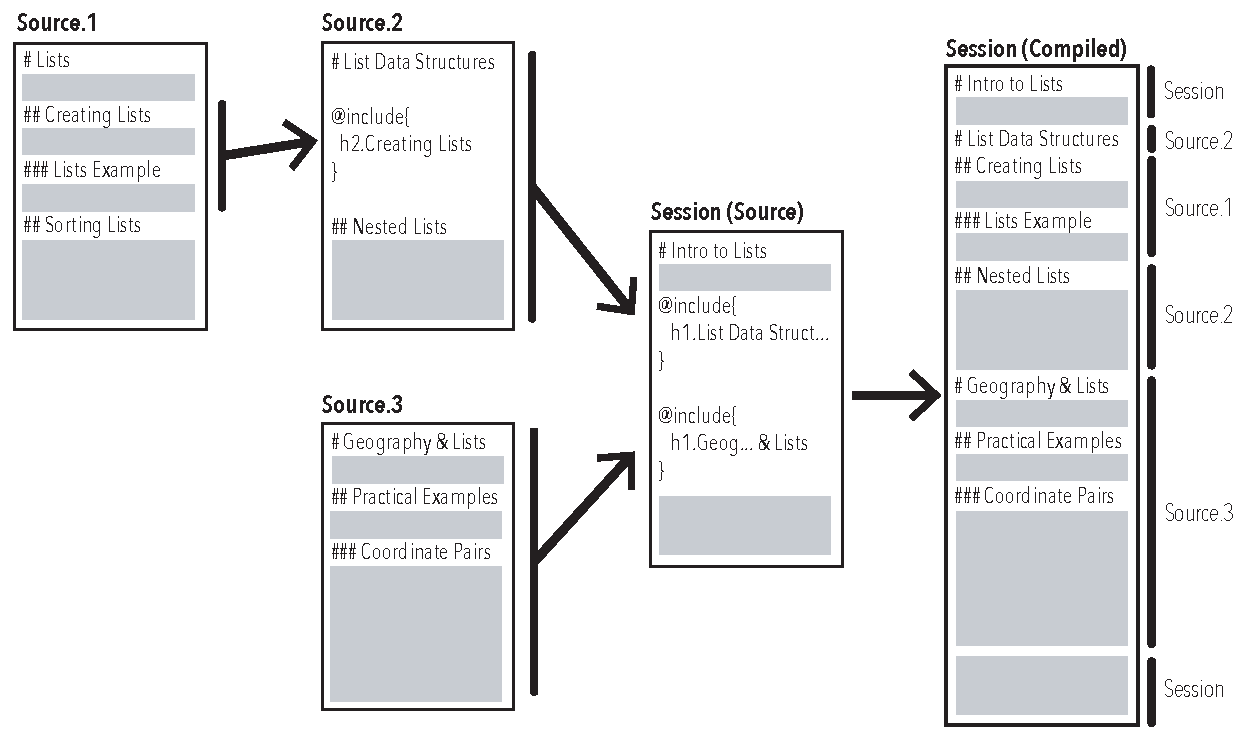
\includegraphics[width=\textwidth, angle=0]{Illustration.pdf}
  \caption{Illustration of \gp Notebook `Compilation' Process}
  \label{fig:Illustration}
\end{figure}

Finally, in order to manage all of this output we make use of Git and the GitHub
web platform to monitor, approve, and roll back alterations to any submitted
revisions to \gp Atoms, Sessions, or Modules. This provides additional
capabilities such as allowing an instructor to `fix' their course to a
particular version of an Atom (a `release' or `tag' in Git) such that
development of the Atom by others can continue without the instructor having to
worry that the explanation or code upon which they rely will suddenly change!
Git also gives us the contributor information that we can propagate into
compiled notebooks so that credit is retained, and users and institutions can
better-understand the extent to which \gp is a \emph{joint} project relying on
the contributions of many teachers and developers.

\subsection{Syntax}\label{syntax}

The final element of \gp is necessarily a syntax for specifying how Sessions and
Modules should be compiled from Atoms. We've noted the technical mechanism, as
well as the mapping between markdown and \textsc{html} formatting, above but how
do we select some mix of code and markdown material in one notebook to be
incorporated into another? And how do we do this in a way that is both simple to
express and able to resolve ambiguity? Fortunately, such a model already exists
and was hinted at in Figure \ref{fig:Illustration}: Cascading Style Sheets
(\textsc{css}) uses well-understood `selectors' to specify one or more elements
on a web page to which a set of presentational styles should be applied: an `h1'
in a style sheet indicates that all level 1 headers should observe the styling
rules declared immediately afterwards; while `h1.important' specifies that only
a level 1 header of the class `important' should be selected. More powerfully,
`h1.important a.super' selects \emph{only} anchors of the class `super' that
fall `within' (or `under', if you prefer') a level 1 header of the `important'
class.

What is particularly elegant about this approach is that it provides a means for
selecting and styling multiple pieces of content in the document in one
declaration (where this is desirable) \textit{and} a means for disambiguating
content with the same name but in different positions within a document's
hierarchical structure (where it is not). We have essentially repurposed
\textsc{css} as a means of selecting and importing content from one notebook
into another! Unfortunately, the nature of Jupyter notebooks does not allow this
to happen dynamically at run-time, but it does allow something similar to happen
when an instructor is `compiling' new Sessional and Module content. In short,
the instructor writes whatever content they wish but, using syntax similar to
the examples below, wherever they want to incorporate contributed content from
\gp (or elsewhere) they have only to write an `include' statement to select and
import sections of another notebook. This approach also works recursively: a
notebook can include content from a notebook that itself includes content from
another notebook\ldots

Adopting the language used above: we envision an Atom as a short notebook
focussing on a single concept or method (\eg lists, object-oriented design, or
spatial autocorrelation); some or all of each Atom can then be selected and
imported into a Session, which is itself a notebook; and the sessions can then
be selected and managed through a Module, which can be a notebook or a set of
notebooks. This process is initiated by the instructor creating a blank text
cell in a Jupyter notebook and writing an `include' statement. The statement
should be the \textit{only} content in the cell since \gp will be replacing the
cell with an unknown number of whole text and code cells from the referenced
notebook.

Crucially, `include' statements can be freely intermingled with the instructor's
own content, allowing the instructor to `frame' the concepts in a way that suits
their teaching style but which saves them having to reinvent the wheel for each
class. A Session tackling standardisation could include elements of the relevant
Atom from \gp while still allowing the instructor to interject comments,
observations, questions, and additional tasks to ground the learning experience
in the local context (individual, institutional, etc.). To illustrate this more
clearly, an Atom on Python's approach to dealing with lists could be
incorporated into a longer Session as follows:

\begin{Verbatim}[fontsize=\small]
@include {
    'nb'     = 'http://geopyter.org/atoms/fundamentals/lists.ipynb',
    'select' = 'h1.Understanding Lists'
}
\end{Verbatim}

The `nb' is the path---local or remote---to a valid Jupyter notebook from which
the Session or Module developer wants to import content. The `select' parameter
specifies a selector for which the \gp tool will search within the source
notebook. All content from that point onwards \emph{up to the next selector at
the same level} will the then be copied into the compiled notebook. In example
above, if there were a following h1 covering, for example, `List Operators' then
this would \emph{not} be included because, from a structural standpoint, it is
of equal importance (at the same level in the hierarchy) to `Understanding
Lists' but has \emph{not} been selected. Furthermore, any h2 or h3 subsections
within the `Understanding Lists' section \textit{would} be included since they
are presumed to be providing pedagogical and logical structure to the
Understanding Lists section and so should be carried over.

Clearly, an instructor might want to import only part of of a section, or to
suppress a subsection falling in the middle of a larger resource. In
anticipation of this need, more complex `include' statements with no equivalent
in \textsc{css} are also possible:

\begin{Verbatim}[fontsize=\small]
@include {
    'resource' = 'http://geopyter.org/atoms/fundamentals/lists.ipynb',
    'select' = 'h1.Understanding Lists -h3.Lists Example; h1.Using Lists -h3.Another Example'
}
\end{Verbatim}

In this second example, two level 1 section are imported at the same time (the
selections are separated with semi-colons) and a level 3 subsection from
\emph{within} each of those sections is suppressed using the `-' syntax to
indicate that the section should be removed. An additional difference from true
\textsc{css} is that we allow spaces in the `selector' because we felt that
asking teachers to translate between a natural language header (``Understanding
Lists'') and what \textsc{css} would consider a safe header
(``Understanding\_Lists'') would detract from ease-of-use. A second departure
from the \textsc{css} standard is that selectors are not separated with commas:
we wanted to allow for this punctuation to be part of a section heading and felt
that semi-colons are rather more rare in that context.

\section{Use Cases}\label{uses}

Two use-cases: an online module of eight sessions, and an in-person module
lasting one semester might serve to further illustrate how this approach offers
a substantively new way to think about teaching programming material more
generally.

\subsection{An Online Module}\label{an-online-module}

There has been increasing interest at universities in Massive Open Online
Courses, or \textsc{mooc}s, as vehicles for expanding access to higher education
through online delivery. For HE managers, the \textsc{mooc} promises both
enhanced revenue---depending on the model this implies either more people paying
to take the modules or more paying for a certificate of completion at the
end---and enhanced access as people who would be unable to attend the university
in person are nonetheless able to pursue a degree. Our own experience suggests
substantial student interest in `computational social science'
\citep{Lazer2009}, with international students being the most keen on such
modules as they are seen to provide marketable skills (programming) for
graduates from a discipline (geography) with generally high employment rates
(see \citeauthor{rgs2017} \citeyear{rgs2017}).

Whatever the motivation, while expanding access to, and enrolment by, students
is probably a `good thing', the process for developing a new online module or
`converting' an existing face-to-face module to an online format remains far
from easy. Typically, this step requires significant effort and investment by
both the instructor and their institution: all course materials need to be
online, recordings/videos of the lecturer presenting a key concept need to be
made, the sessions need to be `chunked' so that a 3-hour practical becomes
something more manageable, and assessments often need to be substantively
redesigned.

\gp significantly reduces the overhead of several of these stages: rather than
focussing on tasks such as how to explain or illustrate a particular concept,
the instructor can focus the \emph{majority} of their effort on constructing the
type of richer, fuller narrative that \textsc{mooc}s seem to require to engage
students working remotely. If the instructor isn't there to ask questions and
probe student learning on the spot, then the `frame' for each session (as well
as for the module as a whole) becomes crucial as it helps to anchor student
learning in concrete outcomes and encourages them to reflect upon, and
integrate, their progress over the self-guided learning process.

\subsection{In-Class Delivery}\label{in-class-delivery}

In a more traditional in-person format, \gp could be employed differently: since
the instructor is able to interactively provide the `frame' or `scaffold' (see
relevant discussion of `hypermedia' in \citealp{Azevedo2008}) upon which the
learning is built, there is less need for a narrative around each task or weekly
session. Here, the instructor might simply import a group of atoms to cover a
set of concepts and step through them interactively with the students. The
session could wrap up with a targeted project or mini-assessment that requires
the students to translate the concepts into a new problem domain or investigate
the process in more detail: \emph{e.g.} ``we've seen how we can use pandas and
bokeh to analyse demographic groups in London, here's a link to the open data
store page for Phoenix with similar data\ldots{}'' or ``Do you think that
socioeconomic class is a useful metric? Investigate the source of the data we've
just used and see if it squares with your expectations\ldots{}''

In effect, courses built on top of \gp become mash-ups, with the author able to
mix and match atoms as needed for the module objectives, time available, and
level of student. Both sessions and modules are built via composition: atoms are
composed into sessions, sessions into modules. The role of the instructor is
then to provide an integrative narrative that, in a sense, explains their choice
of components. In both the online and offline contexts we think that this has
the potential to free up instructors to concentrate on where they can most
effectively `add value', not in figuring out yet \emph{another} way to explain
how a list or dictionary works, but in explaining why they matter to a
geography, political science, or literature major.

\section{Engagement}\label{engagement}

Because it builds on \textsc{foss} approaches to software development, we expect
\gp to benefit from network effects: the more people use it, the more useful it
becomes, and the more people use it. In common with many such projects we
\emph{do} expect that a relatively small subset of users will contribute the
majority of the content; however, unlike a traditional software project there is
an important role for \emph{teachers}, not just highly-skilled \emph{developers}
and we think that this represents a really exciting opportunity for innovative
new approaches to rise to the surface. There may be only a few who can write the
Python code to conduct a Geographically-Weighted Regression analysis, but it
will be interesting to see how many creative, insightful ways there are to
explain it!

\gp also acknowledges the reality of the need for peer and professional
recognition by incorporating attribution mechanisms through which faculty can be
credited for their work. Contributors can be recognised as the author of content
elements through a Digital Object Identifier (\textsc{doi}), and The \gp team
would also include section editors responsible for the curation of atoms and for
maintenance of official \gp \textsc{doi}s. Instructors who use \gp to compose
sessions or courses can also contribute those modules back to the project and
would also be recognised as the author of record in a similar fashion.
Authorship of \gp educational components, be they atoms, sessions or modules,
provides the contributors with peer-evaluated, impactful materials to add to
their promotion applications.

Although the open source nature of the project means that we cannot strictly
enforce attribution, \gp seeks to make this the easier to do `by default'
through the use of Git to track and insert contributory metadata into the
compiled notebook. We can use this metadata to append a list of contributors to
the end of each notebook, along with any other relevant acknowledgments or
copyright notices. To facilitate re-use while protecting contributions from
unacknowledged exploitation textual content in \gp is covered by a Creative
Commons license; however, to deal with the fact that \gp relies extensively on
open source contributions which are incompatible with some \textsc{cc} licenses
\citep[see discussion in][]{osswatch2013}, code blocks are licensed under the
\textsc{mit} license. The manner in which contributions from authors at
different institutions can be combined also `pollutes' the materials in ways
that inhibit institutional assertions of ownership over \gp content.

\section{Limitations}\label{limitations}

Although we are profoundly excited both by the possibility of shifting to
compositional approaches to content-development, and by the impact that shared
materials could have on our teaching, it is highly unlikely that our first
attempt to divide up the entire field into discrete units of instruction will be
entirely successful. For this, it will be useful to reference documents such as
the \textit{Body of Knowledge} \citep{bok2018} and \textit{Subject Benchmark
Statement} \citep{QAA2014} for the `why' and `what' of instruction, leaving \gp
to deal with the `how'. Moreover, the open source, contributory nature of the
project positions us to build \gp on top of the shared understanding of many
specialists with a range of ideas about how to break apart---and put back
together---the constituent elements of our domain knowledge in ways that speak
to different types of students.

For the time being we have also deliberately hobbled \gp in one important way:
an \texttt{include} command must be in a cell that does not contain any other
text or code. This was done primarily for simplicity: it's a lot easier to look
for whole (text) cells that match a target pattern than to have to try to parse
long blocks of text or code on the off-chance that something might match; it
also avoids any ambiguity as to whether the \texttt{include} is a \gp command or
`real' code as might happen, for instance, if \gp were used with a different
programming language. Not coincidentally, it is also a good deal easier to know
that you are replacing an entire block (the one with an include) with one or
more entire blocks that are a mix of text and code, than trying to work out
whether the block in which an include was found needs to be `closed out' before
the import starts.

\section{Conclusion \& Future Directions}\label{future}

From practical experience, conference presentations, and code we tend to already
know who is a good \emph{programmer} or \emph{theorist}, \gp provides a
mechanism for discovering who is a good \emph{teacher}. Sometimes these
abilities may reside in the same person, but more often we expect that they will
not: the strongest developers tend to be people who have been practicing
software development for many years and, consequently, may have difficulty
communicating their ideas to beginner- or intermediate-level students (or
teachers!). For this reason we see the broad-based community-of-practice aspect
of \gp as integral at all stages of the project: system enhancement, content
development, expanding coverage, and instructional design.

Consequently, \gp has a lot in common---both philosophically and
practically---with the Software Carpentry movement \citep{SCF2016}, and although
we seek to tackle a slightly narrower set of issues with a more re-usable set of
resources, we can take both inspiration and warning from their experience. The
benefit, we think, is that while it is possible to design \gp sessions and
modules that follow the popular `bootcamp' approach to instruction (though see
critique in \citealp{Feldon2017}), we want to enable the \textit{same} content
to be employed in a flexible carpentry format as well as a `normal' classroom or
\textsc{mooc} as required\ldots Or even to enable the instructor to mash all of
those formats together such that they use a `bootcamp' format for the
introduction to Unix and the command line, an online-formatted \gp resource for
foundational concepts in computer science, and a traditional course format for
the (geo)data analysis instruction. All pulled from the same source!

Ultimately, although \gp was developed with teaching needs in mind there is, of
course, no reason why it couldn't be put to other uses: in combination with with
\texttt{nteract} (\url{https://github.com/nteract/nteract}) it would allow
developers or researchers to build fully-fledged applications as scripts
assembled from a collection of notebooks; or as an addition to Netflix's
notebook ecology to allow for enhanced resource-sharing and standardisation
during the development phase before features and interfaces are `fixed' as
libraries \citep{Ufford2018}. Nonetheless, our focus for the time being remains
the cohort of teachers at all levels tasked with introducing programming
material to their students and wondering where to begin. We hope that \gp makes
a valuable contribution to this application domain and look forward to working
with others to roll out a rich, reusable teaching framework.

\bibliographystyle{apacite}
\bibliography{Geopyter.bib}

\end{document}